% !TEX root = ../../../main.tex
% ==============================================================================
% EJERCICIO 1 - PRÁCTICA 8: CONFIABILIDAD
% Ubicación: solutions/practice_08_reliability/exercises/ex_01.tex
% ==============================================================================
\IfFileExists{main.tex}{%
    \documentclass[main.tex]{subfiles}%
}{%
    \documentclass[../../../main.tex]{subfiles}%
}

\begin{document}

\h2{Ejercicio 1}

Considere los siguientes sistemas:

\begin{center}
    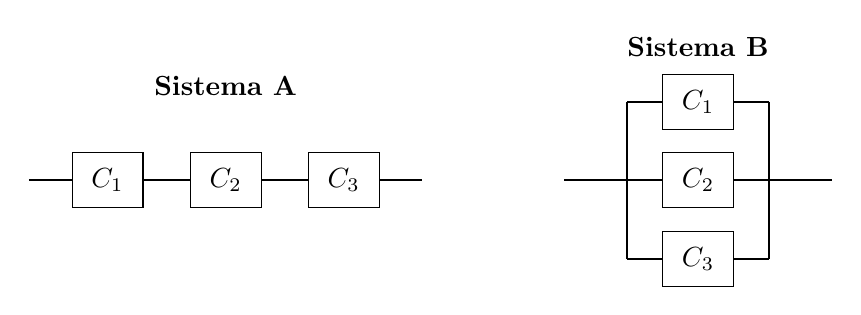
\begin{tikzpicture}[
            bloque/.style={draw=black, fill=white, minimum width=0.9cm, minimum height=0.7cm, font=\bfseries},
            linea/.style={thick, draw=black}
        ]
        % --- SISTEMA A (SERIE) ---
        \node at (1.5, 1.2) {\textbf{Sistema A}};
        \node[bloque] (A1) at (0, 0) {$C_1$};
        \node[bloque] (A2) at (1.5, 0) {$C_2$};
        \node[bloque] (A3) at (3.0, 0) {$C_3$};

        \draw[linea] (-1, 0) -- (A1);
        \draw[linea] (A1) -- (A2);
        \draw[linea] (A2) -- (A3);
        \draw[linea] (A3) -- (4, 0);

        % --- SISTEMA B (PARALELO) ---
        \node at (7.5, 1.7) {\textbf{Sistema B}};
        \node[bloque] (B1) at (7.5, 1.0) {$C_1$};
        \node[bloque] (B2) at (7.5, 0.0) {$C_2$};
        \node[bloque] (B3) at (7.5, -1.0) {$C_3$};

        \draw[linea] (5.8, 0) -- (6.6, 0);
        \draw[linea] (6.6, 1.0) -- (6.6, -1.0);
        \draw[linea] (6.6, 1.0) -- (B1);
        \draw[linea] (6.6, 0) -- (B2);
        \draw[linea] (6.6, -1.0) -- (B3);

        \draw[linea] (B1) -- (8.4, 1.0);
        \draw[linea] (B2) -- (8.4, 0);
        \draw[linea] (B3) -- (8.4, -1.0);
        \draw[linea] (8.4, 1.0) -- (8.4, -1.0);
        \draw[linea] (8.4, 0) -- (9.2, 0);
    \end{tikzpicture}
\end{center}

Asumiendo que cada componente tiene una confiabilidad de $0{,}94$, $0{,}95$ y $0{,}80$, respectivamente, se pide determinar para cada sistema los siguientes aspectos.
\begin{enumerate}[(a)]
    \item Función de confiabilidad.
    \item Función de estructura.
    \item Vectores de camino mínimo.
\end{enumerate}

\h3{Desarrollo}
% Datos iniciales de confiabilidad dados en el problema
Contamos con las confiabilidades individuales de cada uno de los tres componentes independientes:
\begin{equation*}
    R_1 = 0{,}94, \quad R_2 = 0{,}95, \quad R_3 = 0{,}80.
\end{equation*}

Para describir el estado de cada componente, usamos una variable binaria sencilla: $x_i = 1$ si el componente funciona y $x_i = 0$ si falla. El vector de estado del circuito es $\mathbf{x} = (x_1, x_2, x_3)$.

Analizamos ahora cada sistema paso a paso.

\vspace{3mm}
\h3{1. Sistema A (conexión en serie)}

En una conexión en serie, los componentes se ubican uno detrás de otro. El flujo de funcionamiento requiere que todos los componentes estén sanos al mismo tiempo; si uno solo falla, la corriente o señal se interrumpe y todo el sistema se cae.

% Sub-ítem (b): Función de estructura
\h3{(b) Función de estructura}
Para que el sistema se encuentre operativo ($\phi_A(\mathbf{x}) = 1$), es indispensable que los tres componentes funcionen simultáneamente ($x_1 = 1$, $x_2 = 1$ y $x_3 = 1$). Por lo tanto, su función de estructura corresponde al mínimo (o producto) de las variables de estado:
\begin{equation*}
    \phi_A(\mathbf{x}) = \min(x_1, x_2, x_3) = x_1 x_2 x_3.
\end{equation*}

% Sub-ítem (c): Caminos mínimos
\h3{(c) Vectores y conjuntos de camino mínimo}
Un camino mínimo es un conjunto mínimo de componentes indispensables que asegura el funcionamiento del sistema. Al necesitar obligatoriamente a todas las piezas, existe un único vector de camino mínimo:
\begin{equation*}
    \mathbf{x}^{(1)} = (1, 1, 1), \quad \text{con conjunto de camino mínimo } A_1 = \{1, 2, 3\}.
\end{equation*}

% Sub-ítem (a): Confiabilidad
\h3{(a) Función de confiabilidad}
Dado que los componentes operan con total independencia, la probabilidad de que todos funcionen a la vez es el producto directo de sus confiabilidades individuales:
\begin{equation*}
    R_A = R_1 \cdot R_2 \cdot R_3 = 0{,}94 \times 0{,}95 \times 0{,}80 = 0{,}7144 \quad (71{,}44\%).
\end{equation*}

\vspace{3mm}
\h3{2. Sistema B (conexión en paralelo)}

En una conexión en paralelo, los componentes están dispuestos en ramas alternativas. Para que el sistema funcione no necesitamos que operen todos, basta con que al menos uno de ellos esté activo.

% Sub-ítem (b): Función de estructura
\h3{(b) Función de estructura}
Como el sistema se mantiene operativo mientras al menos uno de los tres componentes funcione, su función de estructura es directamente el máximo:
\begin{equation*}
    \phi_B(\mathbf{x}) = \max(x_1, x_2, x_3).
\end{equation*}

% Sub-ítem (c): Caminos mínimos
\h3{(c) Vectores y conjuntos de camino mínimo}
Como cualquier componente que funcione por sí solo mantiene con vida al sistema, cada uno conforma un camino mínimo por separado:
\begin{gather*}
    \mathbf{x}^{(1)} = (1, 0, 0) \implies B_1 = \{1\}, \\
    \mathbf{x}^{(2)} = (0, 1, 0) \implies B_2 = \{2\}, \\
    \mathbf{x}^{(3)} = (0, 0, 1) \implies B_3 = \{3\}.
\end{gather*}

% Sub-ítem (a): Confiabilidad calculada por complemento
\h3{(a) Función de confiabilidad}
Para calcular la confiabilidad de un sistema en paralelo de forma directa, tendríamos que sumar la probabilidad de que funcione exactamente un componente, dos componentes o los tres a la vez, lo cual requiere varios cálculos. Resulta mucho más simple calcularla por el \textbf{evento complementario}: un sistema en paralelo únicamente deja de funcionar en el caso extremo de que \textbf{todos sus componentes fallen al mismo tiempo}.

La probabilidad de que un componente falle es $1 - R_i$. Por la independencia de las componentes, la probabilidad de que las tres fallen simultáneamente es el producto $(1 - R_1)(1 - R_2)(1 - R_3)$.

Por lo tanto, la confiabilidad es simplemente $1$ menos la probabilidad de que fallen todas:
\begin{equation*}
    R_B = 1 - (1 - R_1)(1 - R_2)(1 - R_3) = 1 - (0{,}06 \times 0{,}05 \times 0{,}20) = 0{,}9994 \quad (99{,}94\%).
\end{equation*}


\newpage
\conclusion{El Sistema A en configuración serie ofrece una confiabilidad de $71{,}44\%$, valor que es inferior a la de su componente más débil ($80\%$). Esto ocurre porque la falla de una sola pieza anula todo el circuito. En contraste, el Sistema B en configuración paralelo alcanza una confiabilidad de $99{,}94\%$, muy superior a la de su mejor componente ($95\%$), gracias a la redundancia que ofrecen sus ramas alternativas.}

\end{document}
